\documentclass[aspectratio=169, 10pt]{beamer}

% --- Packages ---
\usepackage[utf8]{inputenc}
\usepackage{tikz}
\usepackage{pgfplots}
\usepackage{amsmath, amssymb, amsfonts}
\usepackage{booktabs}
\usepackage{bm}
\usepackage{xcolor}
\usetikzlibrary{arrows.meta, calc, positioning, shapes.geometric, decorations.pathreplacing, backgrounds, fit, shadows, patterns, shapes.arrows, angles, quotes}
\pgfplotsset{compat=1.17}

% NYU Colors
\definecolor{nyupurple}{RGB}{87,46,140}
\definecolor{nyuheader}{RGB}{172,159,195}
\definecolor{nyufooter}{RGB}{189,178,211}

% Theme
\usetheme{default}
\setbeamertemplate{navigation symbols}{}

% Itemize
\setbeamercolor{itemize item}{fg=nyupurple}
\setbeamercolor{itemize subitem}{fg=nyupurple}
\setbeamercolor{itemize subsubitem}{fg=nyupurple}
\setbeamertemplate{itemize item}{\textbullet}
\setbeamertemplate{itemize subitem}{\textbullet}
\setbeamertemplate{itemize subsubitem}{\textbullet}

% Blocks
\setbeamercolor{block title}{fg=white, bg=nyupurple}
\setbeamercolor{block body}{fg=black, bg=nyuheader!30}
\setbeamercolor{block title alerted}{fg=white, bg=red!70}
\setbeamercolor{block body alerted}{fg=black, bg=red!10}
\setbeamercolor{block title example}{fg=white, bg=green!50!black}
\setbeamercolor{block body example}{fg=black, bg=green!10}

% Diagram colors
\definecolor{darkblue}{RGB}{0,51,102}
\definecolor{brightblue}{RGB}{0,102,204}
\definecolor{lightblue}{RGB}{153,204,255}
\definecolor{darkgreen}{RGB}{0,102,51}
\definecolor{accentred}{RGB}{192,0,0}
\definecolor{accentgreen}{RGB}{0,128,0}
\definecolor{accentorange}{RGB}{255,128,0}

% Commands
\newcommand{\vect}[1]{\boldsymbol{#1}}
\newcommand{\mat}[1]{\mathbf{#1}}

% Header
\makeatletter
\setbeamertemplate{frametitle}{%
    \nointerlineskip%
    \begin{beamercolorbox}[wd=\paperwidth,ht=0.7cm,dp=0.15cm,rightskip=0.5cm]{frametitle}
        \hspace{0.3cm}\usebeamerfont{frametitle}\insertframetitle%
        \hfill%
        \raisebox{0.08cm}{{\bfseries\sffamily\color{nyupurple}NYU}}%
    \end{beamercolorbox}%
}
\makeatother
\setbeamercolor{frametitle}{fg=black, bg=nyuheader}
\setbeamerfont{frametitle}{size=\large}

% Footer
\setbeamertemplate{footline}{%
    \begin{tikzpicture}[remember picture, overlay]
        \fill[nyufooter] ([yshift=0.6cm]current page.south west) rectangle ([xshift=5cm]current page.south east);
        \fill[nyufooter!70] ([yshift=0.6cm, xshift=5cm]current page.south west) rectangle ([xshift=10.5cm]current page.south east);
        \fill[nyufooter!40] ([yshift=0.6cm, xshift=10.5cm]current page.south west) rectangle (current page.south east);
        \node[anchor=west, font=\small] at ([xshift=0.3cm, yshift=0.3cm]current page.south west) {Dr.\ Aliasghar Arab};
        \node[anchor=center, font=\small] at ([yshift=0.3cm]current page.south) {Autonomous Mobile Robots};
        \node[anchor=east, font=\small] at ([xshift=-0.3cm, yshift=0.3cm]current page.south east) {LECTURE 8 -- FALL 2025 \quad \insertframenumber{} / \inserttotalframenumber};
    \end{tikzpicture}%
}

% Title page
\defbeamertemplate*{title page}{customized}[1][]
{
    \begin{tikzpicture}[remember picture, overlay]
        \node[anchor=north east] at ([xshift=-0.8cm, yshift=-0.8cm]current page.north east) {%
            {\bfseries\sffamily\Large\color{nyupurple}NYU}%
            {\sffamily\normalsize\color{black}\ \ TANDON SCHOOL OF ENGINEERING}%
        };
    \end{tikzpicture}
    
    \vspace{2cm}
    \centering
    {\Large\bfseries\inserttitle\par}
    \vspace{0.3cm}
    {\insertsubtitle\par}
    \vspace{1cm}
    {\insertauthor\par}
    \vspace{0.3cm}
    {\small\insertinstitute\par}
    \vspace{0.5cm}
    {\insertdate\par}
}

% Title info
\title{Autonomous Mobile Robots}
\subtitle{Lecture 8: Motion Planning Algorithms}
\author{Dr.\ Aliasghar Arab}
\institute{NYU Tandon School of Engineering}
\date{Fall 2025}

\begin{document}

% Title slide
{
\setbeamertemplate{footline}{}
\begin{frame}[plain]
\titlepage
\end{frame}
}

\begin{frame}{Lecture Overview}
\vspace{0.3cm}

Today's lecture covers the integration of control and planning:

\vspace{0.4cm}

\begin{enumerate}
\item \textbf{Control Philosophy:} Deterministic vs probabilistic approaches

\vspace{0.3cm}

\item \textbf{Nonlinear Model Predictive Control (NMPC):} Optimization and implementation

\vspace{0.3cm}

\item \textbf{Local Planning:} Dynamic Window Approach (DWA)

\vspace{0.3cm}

\item \textbf{Global Planning:} RRT and RRT* algorithms

\vspace{0.3cm}

\item \textbf{System Integration:} Complete autonomous navigation architecture
\end{enumerate}
\end{frame}

\begin{frame}{Project Expectations}
\vspace{0.3cm}

\begin{block}{Three Essential Components}
\textbf{1. System Modeling}

\vspace{0.2cm}

\begin{itemize}
\item Kinematics, dynamics, mathematical formulation
\item Physical working principles and implementation
\end{itemize}

\vspace{0.3cm}

\textbf{2. Control Methodology}

\vspace{0.2cm}

\begin{itemize}
\item Justification of chosen approach
\item Comprehensive testing and validation
\end{itemize}

\vspace{0.3cm}

\textbf{3. Motion Planning}

\vspace{0.2cm}

\begin{itemize}
\item Integration of planning algorithms
\item Explanation of underlying principles
\end{itemize}
\end{block}
\end{frame}

\begin{frame}{Deterministic vs Probabilistic Control}
\vspace{0.3cm}

\begin{alertblock}{Fundamental Philosophy}
Deterministic methods rely on known physics, not probability distributions
\end{alertblock}

\vspace{0.4cm}

\begin{columns}[T]
\begin{column}{0.48\textwidth}
\begin{block}{Deterministic Control (NMPC)}
System model: $\dot{x} = f(x, u)$

\vspace{0.2cm}

\begin{itemize}
\item Physics is reliable and known
\item Future states are predictable
\item Suitable for well-modeled systems
\end{itemize}
\end{block}
\end{column}

\begin{column}{0.48\textwidth}
\begin{block}{Probabilistic Methods (RL)}
System: $P(s'|s, a)$ (MDPs)

\vspace{0.2cm}

\begin{itemize}
\item Environment is uncertain
\item Outcomes are stochastic
\item Optimizes expected reward
\end{itemize}
\end{block}
\end{column}
\end{columns}

\vspace{0.3cm}

\textit{Selection criterion: Confidence in physical model accuracy}
\end{frame}

\begin{frame}{Case Study: Frozen Lake Problem}
\vspace{0.3cm}

\begin{exampleblock}{Stochastic Environment Scenario}
\textbf{Scenario:} Robot navigation on slippery ice

\vspace{0.2cm}

\textbf{Command:} ``Move Forward''

\vspace{0.2cm}

\textbf{Actual outcomes:}

\vspace{0.2cm}

\begin{itemize}
\item 33\% probability: Move Forward
\item 33\% probability: Slide Left
\item 33\% probability: Slide Right
\end{itemize}
\end{exampleblock}

\vspace{0.4cm}

\textbf{Limitation:} NMPC assumes deterministic dynamics

\textbf{Solution:} Reinforcement learning handles probability distributions
\end{frame}

\begin{frame}{NMPC Optimization Formulation}
\vspace{0.3cm}

\begin{block}{Optimal Control Problem}
At each time step $t$, solve over prediction horizon $T_p$:

\vspace{0.3cm}

\[
\min_{u} J = \int_t^{t+T_p} \left[\|x(\tau) - x_{\text{ref}}(\tau)\|^2_Q + \|u(\tau)\|^2_R\right] d\tau + \|x(t+T_p) - x_{\text{goal}}\|^2_P
\]
\end{block}

\vspace{0.4cm}

\textbf{Subject to constraints:}

\vspace{0.2cm}

\begin{itemize}
\item System dynamics: $\dot{x} = f(x, u)$
\item State constraints: $x \in \mathcal{X}_{\text{safe}}$
\item Input constraints: $u \in \mathcal{U}_{\text{feasible}}$
\end{itemize}
\end{frame}

\begin{frame}{Prediction Horizon Concept}
\vspace{0.3cm}

\begin{alertblock}{Prediction Horizon}
$T_p$ determines how far into the future the controller predicts
\end{alertblock}

\vspace{0.4cm}

Key insights:

\vspace{0.2cm}

\begin{itemize}
\item Longer $T_p$ → Better planning, higher computational cost

\vspace{0.2cm}

\item Shorter $T_p$ → Faster computation, more reactive behavior

\vspace{0.2cm}

\item Typical values: 1-5 seconds for mobile robots

\vspace{0.2cm}

\item Must balance prediction quality with real-time requirements
\end{itemize}
\end{frame}

\begin{frame}{Receding Horizon Principle}
\vspace{0.3cm}

\begin{center}
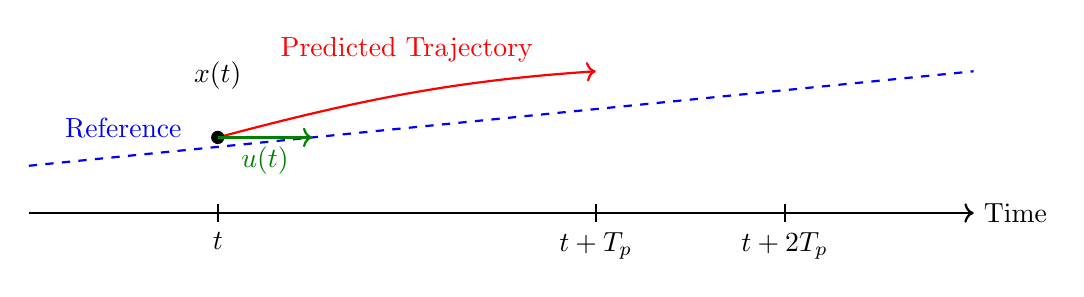
\begin{tikzpicture}[scale=1.2]
% Time axis
\draw[->, thick] (0,0) -- (10,0) node[right] {Time};

% Time markers
\draw[thick] (2,0.1) -- (2,-0.1) node[below] {$t$};
\draw[thick] (6,0.1) -- (6,-0.1) node[below] {$t + T_p$};
\draw[thick] (8,0.1) -- (8,-0.1) node[below] {$t + 2T_p$};

% Reference trajectory
\draw[blue, dashed, thick] (0,0.5) -- (10,1.5);
\node[blue, above] at (1,0.7) {Reference};

% Predicted trajectory
\draw[red, thick, ->] (2,0.8) .. controls (3.5,1.2) and (4.5,1.4) .. (6,1.5);
\node[red, above] at (4,1.5) {Predicted Trajectory};

% Current state
\fill[black] (2,0.8) circle (2pt);
\node[above] at (2,1.2) {$x(t)$};
\draw[->, thick, green!50!black] (2,0.8) -- (3,0.8);
\node[green!50!black, below] at (2.5,0.8) {$u(t)$};
\end{tikzpicture}
\end{center}

\vspace{0.4cm}

\begin{block}{Control Execution}
\textbf{1.} Measure current state $x(t)$ \quad \textbf{2.} Solve optimization over horizon $T_p$ → obtain $u^*(t)$

\textbf{3.} Apply only first control $u^*(t)$ \quad \textbf{4.} Shift window and repeat
\end{block}
\end{frame}

\begin{frame}{Cost Function Components}
\vspace{0.3cm}

\begin{columns}[T]
\begin{column}{0.32\textwidth}
\begin{block}{Tracking Error}
$\|x - x_{\text{ref}}\|^2_Q$

\vspace{0.2cm}

\begin{itemize}
\item Penalizes path deviation
\item Large $Q$: tight tracking
\item Small $Q$: loose tracking
\end{itemize}
\end{block}
\end{column}

\begin{column}{0.32\textwidth}
\begin{block}{Control Effort}
$\|u\|^2_R$

\vspace{0.2cm}

\begin{itemize}
\item Penalizes large inputs
\item Large $R$: smooth control
\item Small $R$: aggressive
\end{itemize}
\end{block}
\end{column}

\begin{column}{0.32\textwidth}
\begin{block}{Terminal Cost}
$\|x(T_p) - x_{\text{goal}}\|^2_P$

\vspace{0.2cm}

\begin{itemize}
\item Ensures final state quality
\item Improves stability
\item Guides to goal region
\end{itemize}
\end{block}
\end{column}
\end{columns}

\vspace{0.4cm}

\begin{alertblock}{Engineering Insight}
Weights $Q$, $R$, $P$ are tuning parameters - balance tracking vs control effort
\end{alertblock}
\end{frame}

\begin{frame}{Real-World Application: Autonomous Racing}
\vspace{0.3cm}

\begin{exampleblock}{Abu Dhabi Autonomous Racing League}
\textbf{Winner:} Technical University of Munich (NMPC implementation)

\vspace{0.2cm}

\textbf{Performance:} 250+ km/h, zero crashes during race

\vspace{0.2cm}

\textbf{Critical:} Tire friction modeling $F_{\text{lateral}} = \mu(v, \alpha) \cdot F_N$
\end{exampleblock}

\vspace{0.5cm}

\begin{alertblock}{Key Insight}
``At 250 km/h, PID is reactive - by the time you see an error, you've already crashed. You NEED prediction.''
\end{alertblock}
\end{frame}

\begin{frame}{Gradient Descent Solver}
\vspace{0.3cm}

\begin{block}{Continuous-Time Update Law}
\[
\dot{u} = -\alpha \nabla J(u) = -\alpha \frac{\partial J}{\partial u}
\]
\end{block}

\vspace{0.4cm}

Understanding the notation:

\vspace{0.2cm}

\begin{itemize}
\item $\dot{u}$ represents \textbf{algorithmic time derivative}

\vspace{0.2cm}

\item Solver ``flows'' down cost surface toward minimum

\vspace{0.2cm}

\item Not physical system time - this is solver iteration
\end{itemize}

\vspace{0.4cm}

\begin{alertblock}{Implementation}
Gradient descent operates in solver time, not physical time
\end{alertblock}
\end{frame}

\begin{frame}{Visualizing Gradient Descent}
\vspace{0.3cm}

\begin{center}
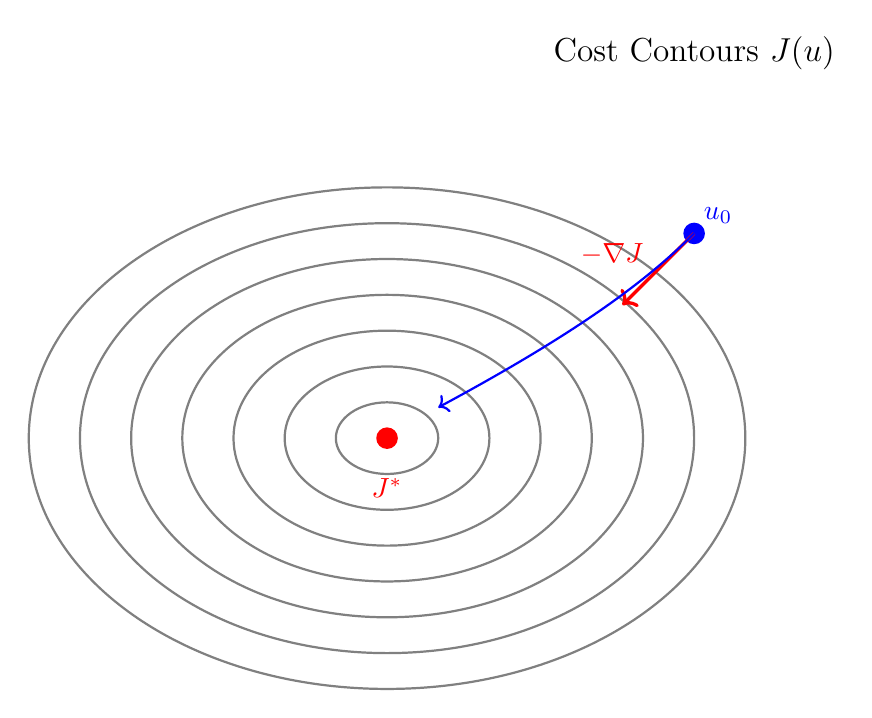
\begin{tikzpicture}[scale=1.3]
% Cost contours
\foreach \r in {0.5, 1, 1.5, 2, 2.5, 3, 3.5}
    \draw[gray, thick] (0,0) ellipse ({\r} and {\r*0.7});

% Minimum
\fill[red] (0,0) circle (3pt);
\node[red, below] at (0,-0.3) {$J^*$};

% Initial point
\fill[blue] (3,2) circle (3pt);
\node[blue, above right] at (3,2) {$u_0$};

% Gradient vector
\draw[->, red, very thick] (3,2) -- (2.3,1.3);
\node[red, above left] at (2.6,1.6) {$-\nabla J$};

% Trajectory
\draw[->, blue, thick] (3,2) .. controls (2.5,1.5) and (1.8,1) .. (0.5,0.3);

\node[above] at (3,3.5) {\large Cost Contours $J(u)$};
\end{tikzpicture}
\end{center}

\vspace{0.3cm}

\begin{block}{Process}
Start with initial guess $u_0$ → Compute gradient direction → 

Step opposite to gradient: $u_{k+1} = u_k - \alpha \nabla J$ → Converge to local minimum
\end{block}
\end{frame}

\begin{frame}{Lyapunov Stability Analysis}
\vspace{0.3cm}

\begin{block}{Proof of Convergence}
\textbf{Step 1 - Lyapunov Candidate:} $V(u) = J(u)$

\vspace{0.3cm}

\textbf{Step 2 - Time Derivative:}
\[
\dot{V} = \frac{dJ}{dt} = \frac{\partial J}{\partial u} \cdot \frac{du}{dt} = \frac{\partial J}{\partial u} \cdot \left(-\alpha \frac{\partial J}{\partial u}\right) = -\alpha \left\|\frac{\partial J}{\partial u}\right\|^2
\]

\vspace{0.3cm}

\textbf{Step 3 - Stability:} $\dot{V} = -\alpha \|\nabla J\|^2 \leq 0$
\end{block}

\vspace{0.4cm}

\begin{alertblock}{Guarantee}
Cost decreases monotonically $\rightarrow$ Solver converges stably
\end{alertblock}
\end{frame}

\begin{frame}{Numerical Gradient Estimation}
\vspace{0.3cm}

\begin{block}{Finite Difference Approximation}
\[
\frac{\partial J}{\partial u} \approx \frac{J(u + \delta u) - J(u)}{\delta u}
\]
\end{block}

\vspace{0.4cm}

\begin{exampleblock}{Implementation Steps}
\textbf{1.} Simulate with $u$, compute $J(u)$

\textbf{2.} Perturb: $u' = u + \delta u$

\textbf{3.} Simulate with $u'$, compute $J(u')$

\textbf{4.} Gradient: $\nabla J \approx \frac{J(u') - J(u)}{\delta u}$

\textbf{5.} Update: $u_{\text{new}} = u - \alpha \nabla J$
\end{exampleblock}

\vspace{0.3cm}

\begin{alertblock}{Critical Parameter}
$\delta u$ must be small but not too small (typical: $10^{-6}$)
\end{alertblock}
\end{frame}

\begin{frame}{Critical Simulation Rule}
\vspace{0.3cm}

\begin{alertblock}{10$\times$ Bandwidth Rule}
\[
\Delta t_{\text{sim}} \leq \frac{1}{10} \times \tau_{\text{system}}
\]
\end{alertblock}

\vspace{0.4cm}

\begin{exampleblock}{Practical Example}
\begin{itemize}
\item Motor time constant: $\tau = 0.1$ seconds
\item Required: $\Delta t \leq 0.01$ seconds
\item Prediction horizon $T_p = 2$s $\rightarrow$ 200 simulation steps
\end{itemize}
\end{exampleblock}

\vspace{0.4cm}

\begin{block}{Consequences of Violation}
\begin{itemize}
\item Numerical integration errors
\item Simulation divergence
\item Controller instability
\item ``Robot predicts it's in another country!''
\end{itemize}
\end{block}
\end{frame}

\begin{frame}{Navigation Hierarchy}
\vspace{0.4cm}

\begin{center}
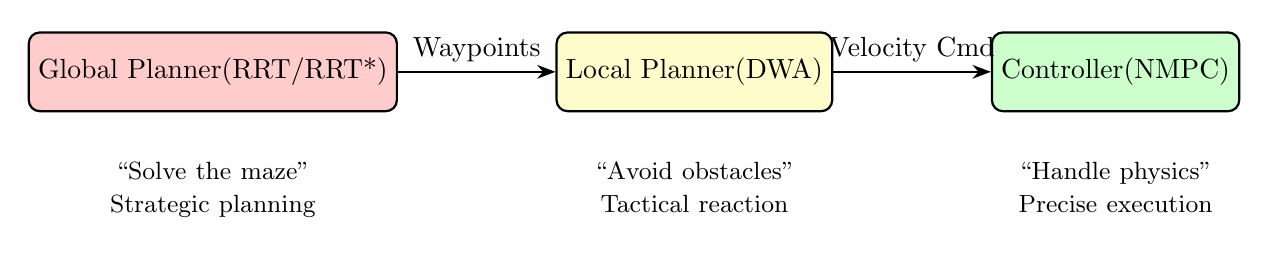
\begin{tikzpicture}[node distance=2cm, auto, >=Stealth, thick]
% Nodes
\node[draw, rectangle, rounded corners, minimum width=3cm, minimum height=1cm, fill=red!20] (global) {Global Planner \\ (RRT/RRT*)};
\node[draw, rectangle, rounded corners, minimum width=3cm, minimum height=1cm, fill=yellow!20, right=of global] (local) {Local Planner \\ (DWA)};
\node[draw, rectangle, rounded corners, minimum width=3cm, minimum height=1cm, fill=green!20, right=of local] (controller) {Controller \\ (NMPC)};

% Arrows
\draw[->] (global) -- node[above] {Waypoints} (local);
\draw[->] (local) -- node[above] {Velocity Cmd} (controller);

% Descriptions below
\node[below=0.5cm of global, text width=3cm, align=center] {\small ``Solve the maze'' \\ Strategic planning};
\node[below=0.5cm of local, text width=3cm, align=center] {\small ``Avoid obstacles'' \\ Tactical reaction};
\node[below=0.5cm of controller, text width=3cm, align=center] {\small ``Handle physics'' \\ Precise execution};
\end{tikzpicture}
\end{center}
\end{frame}

\begin{frame}{Dynamic Window Approach (DWA)}
\vspace{0.3cm}

\begin{block}{Core Principle}
Search in \textbf{velocity space} $(v, \omega)$ instead of position space $(x, y)$
\end{block}

\vspace{0.4cm}

\begin{columns}[T]
\begin{column}{0.55\textwidth}
\begin{block}{Dynamic Window}
\[
V = [V_t - a_{\min} \cdot dt, V_t + a_{\max} \cdot dt]
\]
\[
\Omega = [\omega_t - \alpha_{\min} \cdot dt, \omega_t + \alpha_{\max} \cdot dt]
\]

\vspace{0.2cm}

\begin{itemize}
\item Based on acceleration limits
\item Defines reachable velocities
\item Ensures feasibility
\end{itemize}
\end{block}
\end{column}

\begin{column}{0.40\textwidth}
\begin{exampleblock}{Advantage}
\begin{itemize}
\item Pre-computed trajectories
\item Fast minimization
\item Real-time performance
\end{itemize}
\end{exampleblock}
\end{column}
\end{columns}
\end{frame}

\begin{frame}{Visualizing DWA Search Space}
\vspace{0.3cm}
\centering
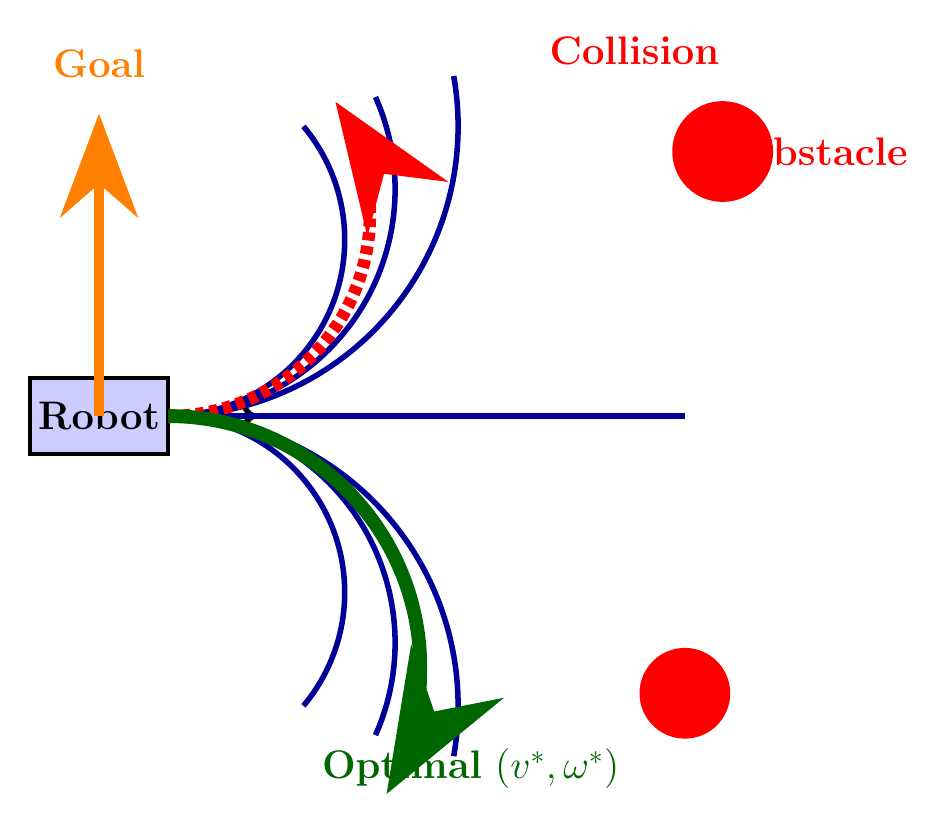
\begin{tikzpicture}[scale=1.6]
% Robot
\draw[fill=blue!20, thick, line width=1.5pt] (0,-0.3) rectangle (1.1,0.3);
\node[font=\Large] at (0.55,0) {\textbf{Robot}};
\draw[->, very thick, line width=2pt] (1.1,0) -- (1.8,0);

% Velocity trajectory arcs - fan of options
\draw[blue!60!black, very thick, line width=2pt] (1.1,0) arc (-90:40:1.4);
\draw[blue!60!black, very thick, line width=2pt] (1.1,0) arc (-90:24:1.8);
\draw[blue!60!black, very thick, line width=2pt] (1.1,0) arc (-90:10:2.3);
\draw[blue!60!black, very thick, line width=2pt] (1.1,0) -- (5.2,0);
\draw[blue!60!black, very thick, line width=2pt] (1.1,0) arc (90:-10:2.3);
\draw[blue!60!black, very thick, line width=2pt] (1.1,0) arc (90:-24:1.8);
\draw[blue!60!black, very thick, line width=2pt] (1.1,0) arc (90:-40:1.4);

% Obstacles
\fill[red] (5.5,2.1) circle (0.4);
\node[red, font=\Large] at (6.3,2.1) {\textbf{Obstacle}};

\fill[red] (5.2,-2.2) circle (0.36);

% Collision trajectory
\draw[red, line width=4.5pt, densely dashed, -{Stealth[scale=2]}] (1.1,0) arc (-90:34:1.6);
\node[red, font=\Large] at (4.8,2.9) {\textbf{Collision}};

% Optimal trajectory
\draw[green!40!black, line width=5pt, -{Stealth[scale=2]}] (1.1,0) arc (90:-30:2);
\node[green!40!black, font=\Large] at (3.5,-2.8) {\textbf{Optimal} $(v^*,\omega^*)$};

% Goal direction
\draw[->, orange, line width=3.5pt, -{Stealth[scale=2]}] (0.55,0) -- (0.55,2.4);
\node[orange, font=\Large] at (0.55,2.8) {\textbf{Goal}};

\end{tikzpicture}
\end{frame}

\begin{frame}{DWA Cost Function}
\vspace{0.3cm}

\begin{block}{Multi-Objective Optimization}
\[
G(v, \omega) = \alpha \cdot \text{Heading}(v, \omega) + \beta \cdot \text{Clearance}(v, \omega) + \gamma \cdot \text{Velocity}(v, \omega)
\]
\end{block}

\vspace{0.4cm}

Component definitions:

\vspace{0.2cm}

\begin{itemize}
\item \textbf{Heading:} Alignment with goal direction

\vspace{0.2cm}

\item \textbf{Clearance:} Distance to nearest obstacle

\vspace{0.2cm}

\item \textbf{Velocity:} Progress toward goal
\end{itemize}

\vspace{0.4cm}

\begin{exampleblock}{Typical Configuration}
10 linear velocities $\times$ 10 angular velocities = 100 trajectories to evaluate
\end{exampleblock}
\end{frame}

\begin{frame}{Rapidly-Exploring Random Trees (RRT)}
\vspace{0.3cm}

\begin{block}{Algorithm}
\textbf{1.} \textbf{Sample:} Random state $x_{\text{rand}}$ in free space

\vspace{0.2cm}

\textbf{2.} \textbf{Nearest:} Find closest node $x_{\text{near}}$ in tree

\vspace{0.2cm}

\textbf{3.} \textbf{Steer:} Extend from $x_{\text{near}}$ toward $x_{\text{rand}}$ by $\Delta q$

\vspace{0.2cm}

\textbf{4.} \textbf{Check:} If collision-free, add $x_{\text{new}}$ to tree

\vspace{0.2cm}

\textbf{5.} \textbf{Repeat:} Until goal reached or maximum iterations
\end{block}

\vspace{0.4cm}

\begin{alertblock}{Key Feature}
Rapidly explores high-dimensional spaces by random sampling
\end{alertblock}
\end{frame}

\begin{frame}{Visualizing RRT Expansion}
\vspace{0.3cm}

\begin{center}
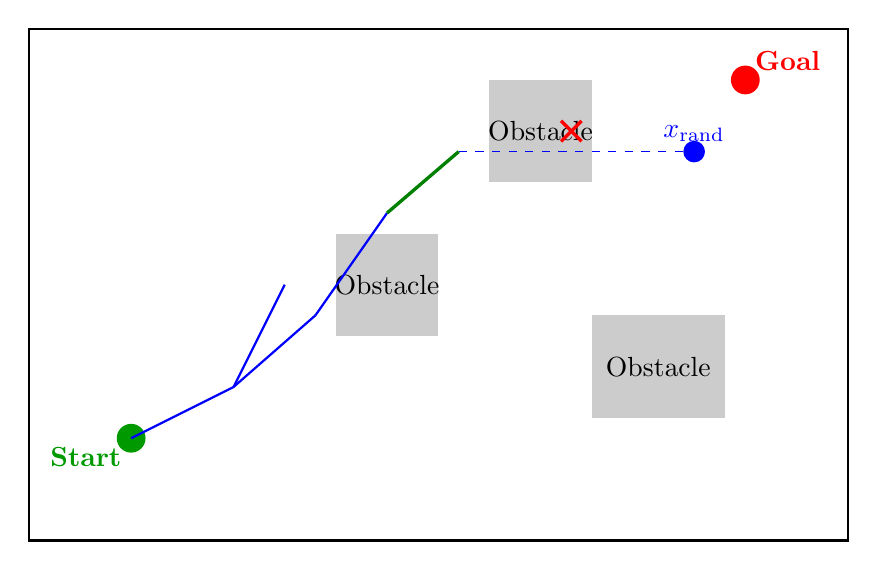
\begin{tikzpicture}[scale=1.3]
% Boundary
\draw[thick] (0,0) rectangle (8,5);

% Obstacles
\fill[gray!40] (4.5,3.5) rectangle (5.5,4.5);
\node at (5,4) {Obstacle};

\fill[gray!40] (3,2) rectangle (4,3);
\node at (3.5,2.5) {Obstacle};

\fill[gray!40] (5.5,1.2) rectangle (6.8,2.2);
\node at (6.15,1.7) {Obstacle};

% Start
\fill[green!60!black] (1,1) circle (4pt);
\node[green!60!black, below left] at (1,1) {\textbf{Start}};

% Goal
\fill[red] (7,4.5) circle (4pt);
\node[red, above right] at (7,4.5) {\textbf{Goal}};

% Tree branches
\draw[blue, thick] (1,1) -- (2,1.5);
\draw[blue, thick] (2,1.5) -- (2.8,2.2);
\draw[blue, thick] (2.8,2.2) -- (3.5,3.2);
\draw[blue, thick] (2,1.5) -- (2.5,2.5);

\draw[green!50!black, very thick] (3.5,3.2) -- (4.2,3.8);

% Random point
\fill[blue] (6.5,3.8) circle (3pt);
\node[blue, above] at (6.5,3.8) {$x_{\text{rand}}$};
\draw[blue, dashed] (4.2,3.8) -- (6.5,3.8);

% Red X on collision
\draw[red, very thick] (5.2,3.9) -- (5.4,4.1);
\draw[red, very thick] (5.2,4.1) -- (5.4,3.9);
\end{tikzpicture}
\end{center}

\vspace{0.3cm}

\begin{block}{Exploration Strategy}
Tree grows toward randomly sampled points, avoiding obstacles
\end{block}
\end{frame}

\begin{frame}{Computational Efficiency: KD-Trees}
\vspace{0.3cm}

\begin{alertblock}{Complexity Challenge}
\begin{itemize}
\item Naive nearest neighbor: $O(N)$ for $N$ nodes
\item With KD-tree: $O(\log N)$ complexity
\item Example: $N = 10{,}000 \rightarrow$ 14 comparisons vs 10,000
\end{itemize}
\end{alertblock}

\vspace{0.4cm}

\begin{block}{KD-Tree Structure}
\begin{itemize}
\item Binary space partitioning
\item Alternating axis splits
\item Essential for real-time RRT
\end{itemize}
\end{block}

\vspace{0.4cm}

\begin{alertblock}{Key Point}
``KD-trees are essential! Without them, RRT is too slow for real-time.''
\end{alertblock}
\end{frame}

\begin{frame}{RRT vs RRT*: Optimality}
\vspace{0.3cm}

\begin{columns}[T]
\begin{column}{0.48\textwidth}
\begin{block}{Standard RRT}
\begin{itemize}
\item Finds \textit{any} feasible path
\item Fast exploration
\item No optimality guarantees
\item Good for: Quick solutions
\end{itemize}
\end{block}
\end{column}

\begin{column}{0.48\textwidth}
\begin{block}{RRT* (Optimal)}
\begin{itemize}
\item Asymptotically optimal
\item ``Rewiring'' improves paths
\item Converges to optimum
\item Good for: Quality paths
\end{itemize}
\end{block}
\end{column}
\end{columns}

\vspace{0.4cm}

\begin{exampleblock}{RRT* Rewiring}
\begin{itemize}
\item Check if $X_{\text{new}}$ provides better paths to neighbors
\item Rewire tree to reduce costs
\item Continuous improvement over time
\end{itemize}
\end{exampleblock}
\end{frame}

\begin{frame}{Complete System Architecture}
\vspace{0.4cm}

\begin{center}
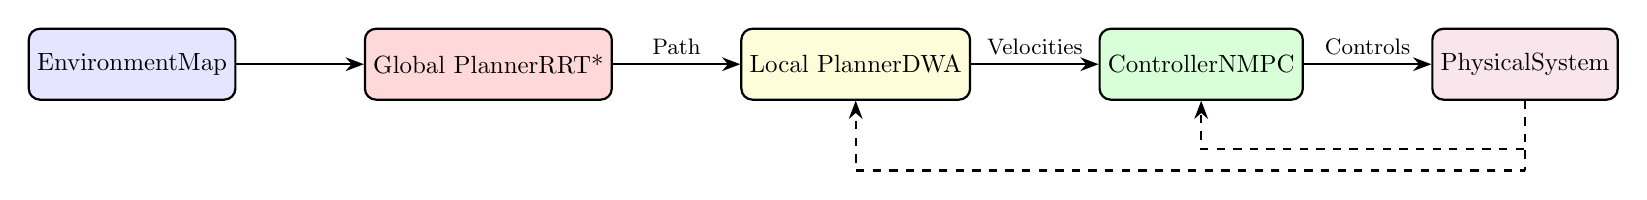
\begin{tikzpicture}[node distance=1.8cm, auto, >=Stealth, thick, scale=0.9, transform shape]
% Nodes
\node[draw, rectangle, rounded corners, minimum width=2.5cm, minimum height=1cm, fill=blue!10] (env) {Environment \\ Map};
\node[draw, rectangle, rounded corners, minimum width=2.5cm, minimum height=1cm, fill=red!15, right=of env] (global) {Global Planner \\ RRT*};
\node[draw, rectangle, rounded corners, minimum width=2.5cm, minimum height=1cm, fill=yellow!15, right=of global] (local) {Local Planner \\ DWA};
\node[draw, rectangle, rounded corners, minimum width=2.5cm, minimum height=1cm, fill=green!15, right=of local] (controller) {Controller \\ NMPC};
\node[draw, rectangle, rounded corners, minimum width=2.5cm, minimum height=1cm, fill=purple!10, right=of controller] (system) {Physical \\ System};

% Forward arrows
\draw[->] (env) -- (global);
\draw[->] (global) -- node[above, font=\small] {Path} (local);
\draw[->] (local) -- node[above, font=\small] {Velocities} (controller);
\draw[->] (controller) -- node[above, font=\small] {Controls} (system);

% Feedback arrows
\draw[->, dashed] (system) |- ++(0,-1.2) -| (controller);
\draw[->, dashed] (system) |- ++(0,-1.5) -| (local);
\end{tikzpicture}
\end{center}

\vspace{0.4cm}

\begin{block}{Integrated Operation}
\begin{itemize}
\item Global planning for strategic navigation
\item Local adaptation for dynamic obstacles
\item Physics-based control for precise execution
\item Continuous sensor feedback for real-time updates
\end{itemize}
\end{block}
\end{frame}

\begin{frame}{Key Technical Insights}
\vspace{0.3cm}

\textbf{1. Deterministic Control Foundation}

\vspace{0.2cm}

\begin{itemize}
\item NMPC relies on accurate physical models
\item Gradient descent with Lyapunov stability guarantees
\item Suitable for well-characterized systems
\end{itemize}

\vspace{0.3cm}

\textbf{2. Critical Implementation Rules}

\vspace{0.2cm}

\begin{itemize}
\item 10$\times$ bandwidth rule: $\Delta t \leq \tau_{\text{system}}/10$
\item Proper finite difference gradient estimation
\item Careful weight selection in cost functions
\end{itemize}

\vspace{0.3cm}

\textbf{3. Hierarchical Planning}

\vspace{0.2cm}

\begin{itemize}
\item Global: RRT/RRT* for strategic paths
\item Local: DWA for dynamic obstacle avoidance
\item Control: NMPC for physics-based execution
\end{itemize}
\end{frame}

\begin{frame}{Practical Implementation Guidelines}
\vspace{0.3cm}

\begin{block}{Development Strategy}
\textbf{1. Start Simple}

\begin{itemize}
\item Basic controller implementation first
\item Incremental complexity addition
\item Early testing and validation
\end{itemize}

\vspace{0.3cm}

\textbf{2. Method Selection}

\begin{itemize}
\item Match complexity to application needs
\item Classical control often sufficient
\item Advanced methods for demanding applications
\end{itemize}

\vspace{0.3cm}

\textbf{3. Validation Process}

\begin{itemize}
\item Comprehensive simulation before hardware
\item Careful time step verification
\item Iterative weight tuning
\end{itemize}
\end{block}
\end{frame}

\begin{frame}{Summary}
\vspace{0.3cm}

Today we covered the complete motion planning pipeline:

\vspace{0.4cm}

\begin{itemize}
\item \textbf{Control philosophy:} When to use deterministic vs probabilistic methods

\vspace{0.3cm}

\item \textbf{NMPC implementation:} Optimization formulation, gradient descent, stability analysis

\vspace{0.3cm}

\item \textbf{Local planning:} Dynamic Window Approach for real-time obstacle avoidance

\vspace{0.3cm}

\item \textbf{Global planning:} RRT/RRT* for strategic path generation

\vspace{0.3cm}

\item \textbf{System integration:} Hierarchical architecture combining all components
\end{itemize}

\vspace{0.4cm}

Next lecture: Advanced topics in perception and sensor fusion
\end{frame}

\begin{frame}{Recommended Resources}
\vspace{0.3cm}

\begin{block}{Reference Materials}
\textbf{Planning Algorithms:} LaValle, ``Planning Algorithms''

\vspace{0.2cm}

\textbf{RRT Foundation:} LaValle (1998)

\vspace{0.2cm}

\textbf{Optimal RRT:} Karaman \& Frazzoli, ``RRT*''

\vspace{0.2cm}

\textbf{Digital Control:} Various sampling theory texts
\end{block}
\end{frame}

\begin{frame}[plain]
\vspace{2cm}
\begin{center}
{\Huge \textbf{End of Lecture 8}}

\vspace{1cm}

{\Large Motion Planning Algorithms}
\end{center}
\end{frame}

\begin{frame}[plain]
\vspace{3cm}
\begin{center}
{\Huge \textbf{Questions?}}
\end{center}
\end{frame}

\end{document}
